\documentclass[border=8pt]{standalone}
\usepackage{pgfplots}
\usepgfplotslibrary{groupplots}
\pgfplotsset{compat=1.18}
\renewcommand{\familydefault}{\sfdefault}
\definecolor{oursline}{HTML}{00747C}
\definecolor{omleline}{HTML}{773588}
\definecolor{ink}{HTML}{17242D}
\definecolor{muted}{HTML}{4A5C67}
\definecolor{gridline}{HTML}{E3EAED}
\begin{document}
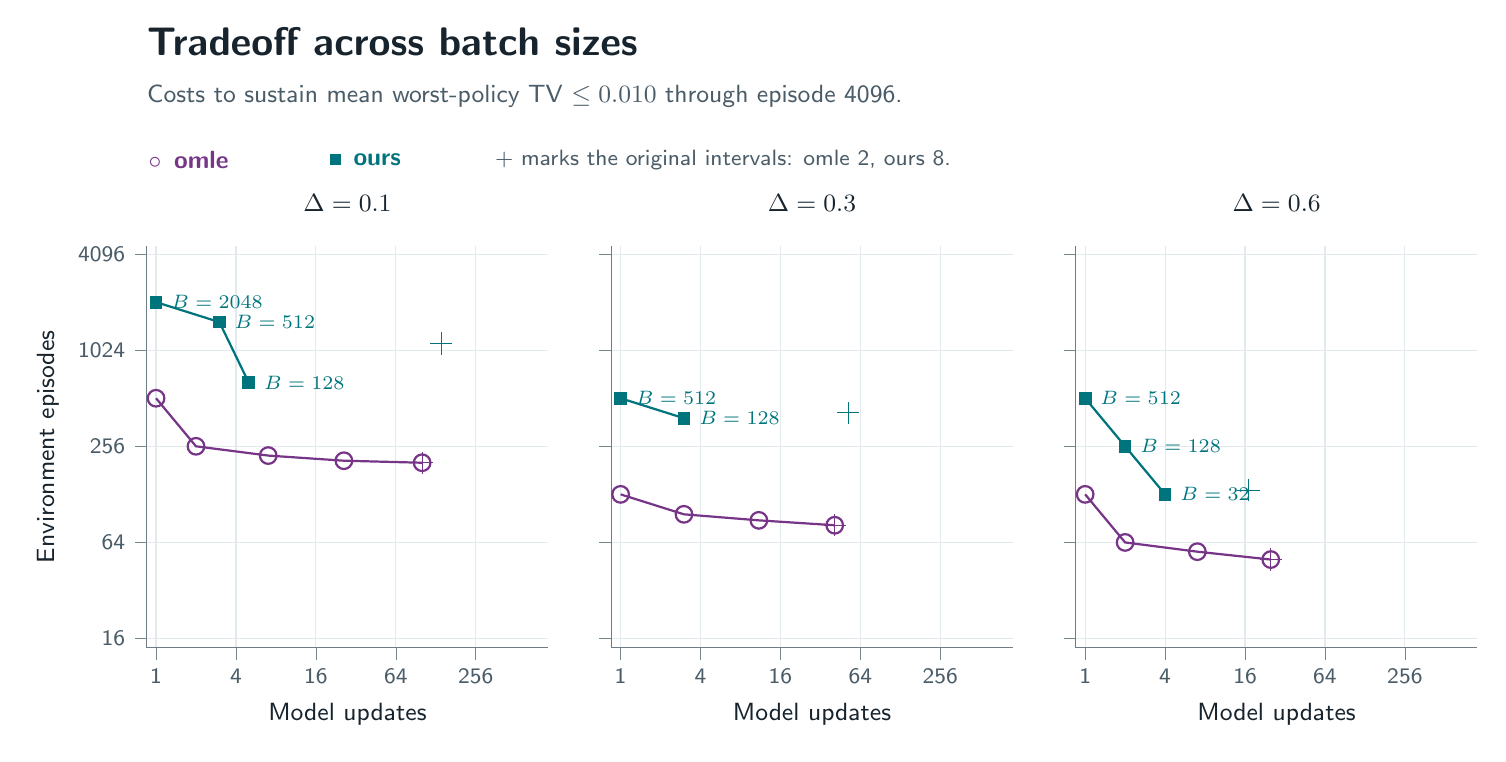
\begin{tikzpicture}[text=ink]
\begin{groupplot}[
  group style={group size=3 by 1,horizontal sep=0.8cm},
  width=5.1cm,height=5.1cm,scale only axis,
  xmode=log,log basis x=2,
  ymode=log,log basis y=2,
  xmin=0.85, xmax=900, ymin=14,
  xtick={1,4,16,64,256},xticklabels={1,4,16,64,256},
  tick align=outside,tick style={muted!75},
  tick label style={font=\footnotesize,text=muted},
  label style={font=\small,text=ink},
  title style={font=\small\bfseries,text=ink,yshift=1mm},
  grid=major,grid style={gridline},
  axis lines*=left,axis line style={muted!80},
  xlabel={Model updates},
  clip=false,
]
\nextgroupplot[title={$\Delta=0.1$},ymax=4587.52,ytick={16,64,256,1024,4096},yticklabels={16,64,256,1024,4096},ylabel={Environment episodes}]
\addplot[omleline,thick,mark=o,mark size=3pt] coordinates {(1,512) (2,256) (7,224) (26,208) (101,202)};
\addplot[only marks,omleline,mark=+,mark size=4pt] coordinates {(101,202)};
\addplot[oursline,thick,mark=square*,mark size=1.9pt] coordinates {(1,2048) (3,1536) (5,640)};
\node[anchor=west,xshift=2pt,font=\scriptsize,text=oursline] at (axis cs:5,640) {$B=128$};
\node[anchor=west,xshift=2pt,font=\scriptsize,text=oursline] at (axis cs:3,1536) {$B=512$};
\node[anchor=west,xshift=2pt,font=\scriptsize,text=oursline] at (axis cs:1,2048) {$B=2048$};
\addplot[only marks,oursline,mark=+,mark size=4pt] coordinates {(141,1128)};
\nextgroupplot[title={$\Delta=0.3$},ymax=4587.52,ytick={16,64,256,1024,4096},yticklabels={}]
\addplot[omleline,thick,mark=o,mark size=3pt] coordinates {(1,128) (3,96) (11,88) (41,82)};
\addplot[only marks,omleline,mark=+,mark size=4pt] coordinates {(41,82)};
\addplot[oursline,thick,mark=square*,mark size=1.9pt] coordinates {(1,512) (3,384)};
\node[anchor=west,xshift=2pt,font=\scriptsize,text=oursline] at (axis cs:3,384) {$B=128$};
\node[anchor=west,xshift=2pt,font=\scriptsize,text=oursline] at (axis cs:1,512) {$B=512$};
\addplot[only marks,oursline,mark=+,mark size=4pt] coordinates {(52,416)};
\nextgroupplot[title={$\Delta=0.6$},ymax=4587.52,ytick={16,64,256,1024,4096},yticklabels={}]
\addplot[omleline,thick,mark=o,mark size=3pt] coordinates {(1,128) (2,64) (7,56) (25,50)};
\addplot[only marks,omleline,mark=+,mark size=4pt] coordinates {(25,50)};
\addplot[oursline,thick,mark=square*,mark size=1.9pt] coordinates {(1,512) (2,256) (4,128)};
\node[anchor=west,xshift=2pt,font=\scriptsize,text=oursline] at (axis cs:4,128) {$B=32$};
\node[anchor=west,xshift=2pt,font=\scriptsize,text=oursline] at (axis cs:2,256) {$B=128$};
\node[anchor=west,xshift=2pt,font=\scriptsize,text=oursline] at (axis cs:1,512) {$B=512$};
\addplot[only marks,oursline,mark=+,mark size=4pt] coordinates {(17,136)};
\end{groupplot}
\node[anchor=west,inner sep=0pt,font=\Large\bfseries] at ([yshift=26mm]group c1r1.north west) {Tradeoff across batch sizes};
\node[anchor=west,inner sep=0pt,text=muted,font=\small] at ([yshift=19mm]group c1r1.north west) {Costs to sustain mean worst-policy TV $\leq 0.010$ through episode 4096.};
\node[anchor=west,font=\small,text=omleline] at ([xshift=-1mm,yshift=11mm]group c1r1.north west) {$\circ$\enspace\textbf{omle}};
\node[anchor=west,font=\small,text=oursline] at ([xshift=22mm,yshift=11mm]group c1r1.north west) {\rule{4pt}{4pt}\enspace\textbf{ours}};
\node[anchor=west,font=\footnotesize,text=muted] at ([xshift=43mm,yshift=11mm]group c1r1.north west) {$+$ marks the original intervals: omle 2, ours 8.};
\end{tikzpicture}
\end{document}
